In order to add high-level autonomous aerial vehicle support to the simulation environment, we used the AirSim \cite{ShahAirSim:Vehicles} plugin for UE4. A table of candidates that were considered is shown in table \ref{table:SimulatorComparison}. We chose to use AirSim with UE4 over other simulation technologies for the following reasons:


\begin{itemize}
\item The design process of the physical environment could be decoupled from the plugin and other plugins could add further functionality independently of AirSim. This meant that new versions of AirSim could be seamlessly integrated with the existing simulation.

\item UE4 has ample documentation and is highly suited to simulating physical phenomena.

\item AirSim has high-level, extensible navigation and sensor APIs for multiple programming languages.

\item AirSim provides the ability to run multiple RAVs and RGVs in the same environment.

\item AirSim has been open-sourced with an MIT licence and was designed to be easily extended.

\item AirSim  provides an API to render unmodified images, depth maps and segmented images.

\item AirSim is highly modular in its approach to modelling sensors and actuators, which means that it can easily be extended with domain-specific functionality.

\item AirSim supports flight controller firmware such as PX4, ROSFlight and Hackflight with minimal setup.

\end{itemize}
AirSim internally models RAVs using different low-level modules outlined in \cite{Shah2017AirSim:Vehicles}. Figure  \ref{fig:AirSimArchitecture} provides an overview of how the different components of the simulator work together.

\begin{figure}
    \centering
    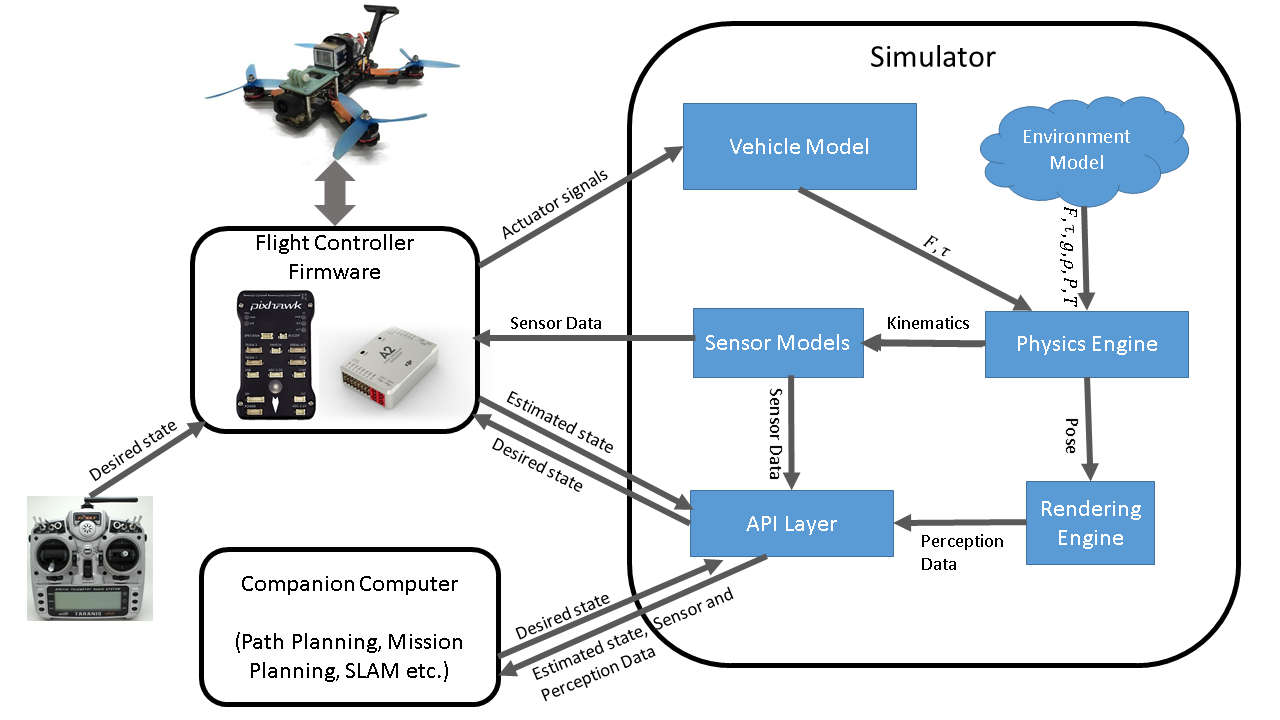
\includegraphics[width=0.5\linewidth]{Chapters/SimulationEnv/Figs/AirSimArchitecture/AirSimArchitecture.png}
    \caption{The architecture of the AirSim simulator. Diagram taken from \cite{Shah2017AirSim:Vehicles}}
    \label{fig:AirSimArchitecture}
\end{figure}

Details of how to integrate AirSim into a custom UE4 project can be found %https://microsoft.github.io/AirSim/docs/unreal_custenv/.
\note{It might be worth discussing how airsim actually models the state of the drone and its ability to integrate with PX4 over mavlink}. Once the plugin had been successfully integrated into the project, some additional functionality was added to meet some of the design objectives, described in the subsequent section.

\subsection{Modifications and Extensions}
\note{Debugging lines added to API, additional cameras added, Radiation simulator and simulated detector added, battery simulator added, on-screen debugging messages added, gps-to-NED conversion tools, debugging lines to show where drones have gone as well as planned routes.}

\subsubsection{Debugging Lines}
\begin{wrapfigure}{r}{0.4\textwidth}
    \centering
    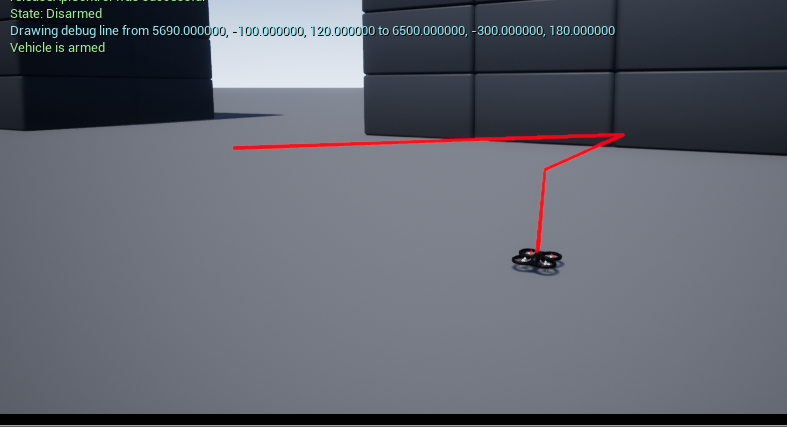
\includegraphics[width=0.4\textwidth]{Chapters/SimulationEnv/Figs/DebuggingLines/DebugLines.png}
    \caption{Debugging Lines Visualise planned UAV route.}
    \label{fig:DebuggingLines}
\end{wrapfigure}
The first modification made to AirSim was to extend the API to allow the user to visualize planned routes using debugging lines. This functionality had already been requested in multiple Github issues \note{do i need to provide links?} and since we also wanted the functionality, we decided to add this to the AirSim API. The end result can be seen in figure \ref{fig:DebuggingLines}. In order to add this functionality, it was necessary to fully understand the architecture of the AirSim simulator and how to expose internal state through its APIs.

As shown in figure \ref{fig:AirSimArchitecture}, AirSim maintains some internal state related to the vehicles that it is simulating and exposes this state through an API layer. In practice, this means that adding functionality to the API layer invloves modifying the underlying levels as well.


